\section{User Study Methodology}
We held a within-subject study with 8 participants at a large Midwestern university in the United States of America during December of 2024 (Figure \ref{fig:studyFlow}). In this section, we describe the process of recruitment and human-subject evaluation for \visowel{} and audio-only pronunciation practice. We ran two pilot sessions before our study, thus participant numbers start from 2.

\subsection{Recruitment}
\begin{table}[t]
    \centering
    \begin{tabular}{l|lllll|}
        ID  & Word List  & 1st Tool & 2nd Tool & Sex \\ \hline
        % P1 & first & Vowel & Control & Male \\ 
        P2 & first & Control & Vowel & Male \\ 
        P3 & second & Vowel & Control & Female \\ 
        P4 & second & Control & Vowel & Female \\ 
        P5 & first & Control & Vowel & Male \\ 
        P6 & second & Control & Vowel & Male \\ 
        P7 & first & Vowel & Control & Female \\ 
        P8 & second & Vowel & Control & Male \\
        P9 & second & Vowel & Control & Female
    \end{tabular}
    \caption{Participant information}
    \label{tab:participants}
\end{table}

We recruited participants through the campus e-newsletter, and physical posters throughout campus buildings (See Table \ref{tab:participants}). The participants were between the ages of 18 and 24, had no history of speech or auditory impairment, and spoke American English as their first language. We limited participants to those who had not spent more than a semester in college learning Spanish, a week studying Spanish in a Spanish-speaking country, or two months in a Spanish-speaking country. We asked participants to choose the sex of the Spanish speaker with which they wished to practice.

\begin{figure*}[ht]
    \centering
    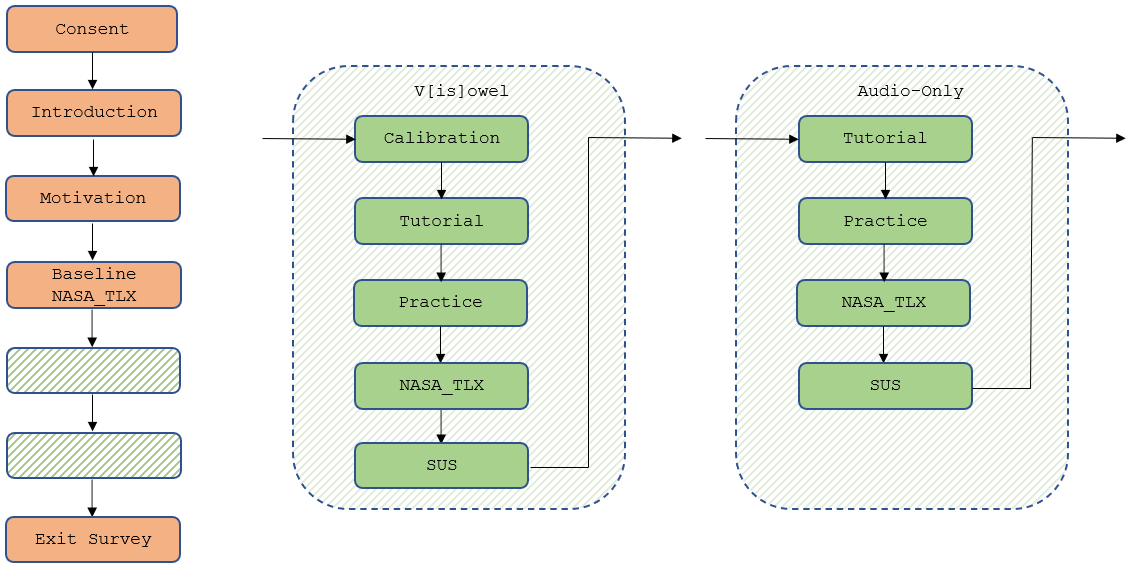
\includegraphics[width=0.8\linewidth]{pictures/workflows/studyFlowNoEval.png}
    \caption{A flowchart representing the progress of the study. The orange boxes represent the fixed portions of the study, the two green striped boxes are the counterbalanced pronunciation practice tools, \visowel{} and audio-only.}
    \label{fig:studyFlow}
\end{figure*}
\subsection{Interface Evaluation}

% study design
To understand how participants process their pronunciation during practice with and without a visualization, we conducted one-hour think-aloud experiments in-person on campus. During the practice portion of the experiment, we often prompted them to express why they decided to record a second time. We randomized the order in which participants saw the two practices, \visowel{} and audio-only (Figure \ref{fig:pracPages}). Since we wanted to test the robustness of our signal processing algorithm and visualization, participants practiced with words that included vowels in varied linguistic contexts. These lists were also counterbalanced to appear with both visualizations. 

% we did not have time to 
% In order to see if either visualization had an effect on pronunciation or perception, participants completed 3 pronunciation and perception evaluations of Spanish words. Before, between, and after interaction with \visowel{} and audio-only feedback.

\subsection{Experimental Setup}
Figure \ref{fig:studyFlow} shows the flow of our study. We collected consent, gave a brief introduction to the project, and had participants record English words for a baseline task load (NASA-TLX). Depending on which condition they saw first, the next step was interaction with \visowel{} or audio-only. Audio-only's interface was identical to \visowel{} without a vowel chart (Figure \ref{fig:audioPrac}). The tutorial for audio-only was a spoken introduction to its mimicry setup. Other than an initial calibration step, interactions with the tools followed the same steps: a tutorial introducing the practice, practice with the tool with four different Spanish minimal pairs, followed by a NASA-TLX and System Usability Score (SUS) surveys. After interacting with both tools, we held a semi-structured exit interview. 

% Once participants practice four different minimal pairs, they fill out the NASA-TLX and SUS surveys, which measure the task load and system usability respectively~\cite{hart1986nasa}. The former measures how laborious practicing pronunciation is while the latter helps explain if that labor is due to the difficulty of processing audio and visual data or to the general usability of the system. 

We ran the tools locally on a Lenovo laptop with a Bluetooth microphone recording at 48kHz. The microphone was set on a \~6" stand. Participants were compensated for their time and effort by a \$20 Amazon gift card. They viewed the interface either on a monitor or laptop screen and used a mouse to navigate the interface. 

After explaining and signing the consent form, we briefly introduced the goal of the project. We used NASA TLX to measure workload~\cite{hart1986nasa}, which measures the workload based on mental, physical, and temporal demand as well as performance, effort, and frustration while doing a task. We took a baseline workload assessment to mitigate potential effects of participant, meeting time, location, and screen difference. Participants were asked to separately record three English words as the baseline assessment. We used the process as a baseline since it would show how difficult participants found it to record and speak on our platform without the mingled effect of practicing pronunciation.  
Then, we introduced the tools to the participants and asked that they let us know if they had any questions before they began. The audio-only introduction was verbal, while the introduction to \visowel{} began with calibration and a 6-step tutorial. After the tutorial, they took a 3-question vowel-chart literacy check. We used the check to allow participants to apply what they'd learned and ask clarification questions about the visualization.

We wrapped up the experiment with a semi-structured survey about their experience using both pronunciation practice tools.

\subsection{Data Analysis}
One person on the research team transcribed the interviews and coded the discussions. In the first round of coding, they marked statements as either relating to pronunciation, visual information, auditory feedback, or reaction to the system. During the second round, they broke up the main codes into sub-codes, which are presented in results. We discovered two main themes during analysis of the coded interview data: the role of \textbf{auditory feedback} in understanding speech with and without visual feedback and how \textbf{visual feedback} can help and confuse learners in their goal to improve pronunciation. 